%====================================================================
\frame{ \frametitle{Joint, Marginal, Conditional} \label{app:JointMargCond}

  \paragraph{Reminder:} 2 loci with 2 alleles each: $(A, a)$, $(B, b)$
  \begin{itemize}
   \item Joint distribution: 
   $$
   \begin{array}{c|cc|c}
   & B & b & \text{marginal}\\
   \hline
   A & f_{AB} & f_{Ab} & p_A = f_{AB} + f_{Ab} \\
   a & f_{aB} & f_{ab} & p_a = f_{aB} + f_{ab} \\
   \hline
   \text{marginal} & q_B = f_{AB} + f_{aB} & q_b = f_{Ab} + f_{ab} & 1 
   \end{array}
  $$ \\ ~
  \item Marginal distribution: 'integrates out' the allele of the other locus
  $$
  \Pr\{B\} = q_B = f_{AB} + f_{aB}
  $$ \\ ~
  \item Conditional distribution
  $$
  \Pr\{A \gv b\} = \frac{\Pr\{A, b\}}{\Pr\{b\}} = \frac{f_{Ab}}{q_b} = \frac{f_{Ab}}{f_{Ab} + f_{ab}}
  $$
  \end{itemize}

}

%====================================================================
\frame{ \frametitle{Posterior distribution and CI (slide \# \ref{sec:CI})} 

  The same holds for combination of parameters, e.g.
  $$
  \delta =  \theta_2 - \theta_3
  $$
  
  $$
  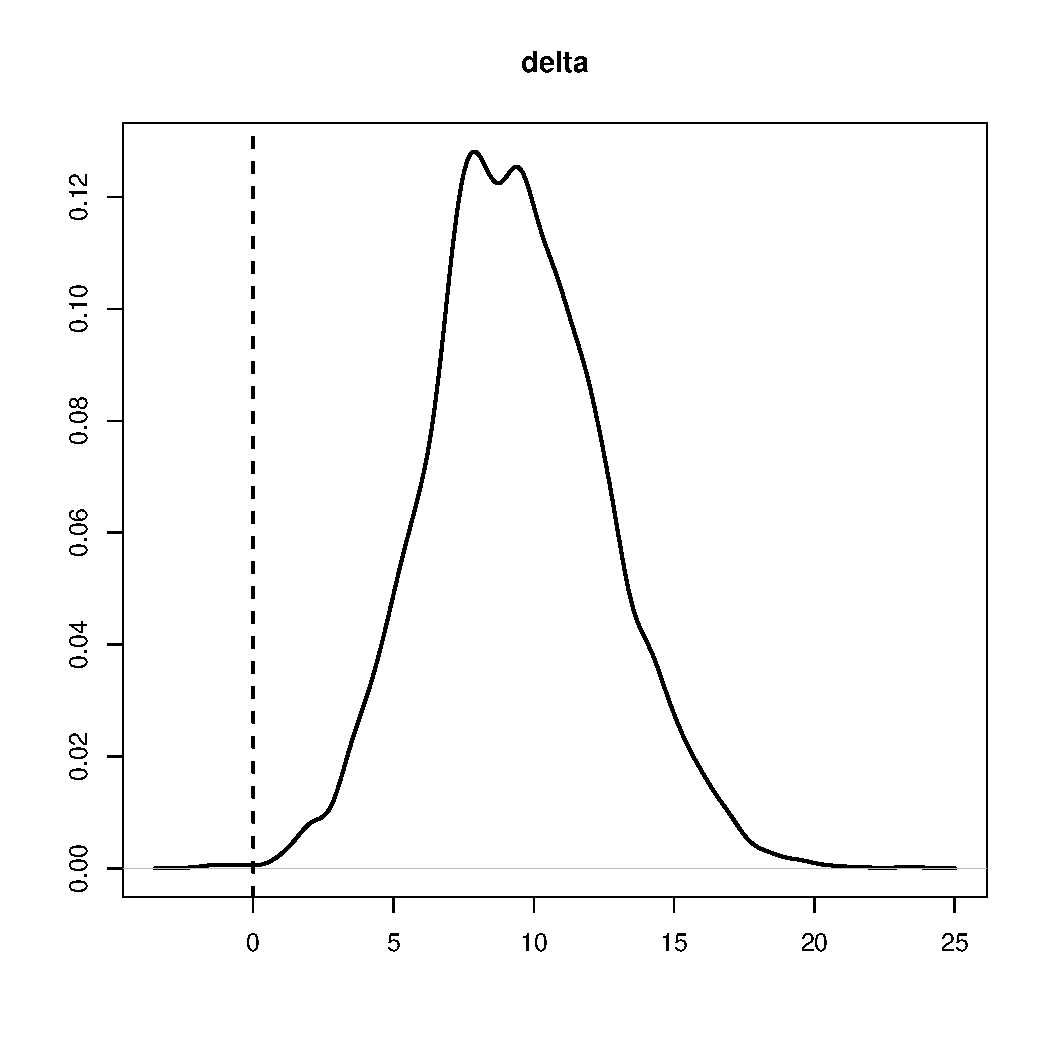
\includegraphics[width=.4\textwidth, height=.4\textheight]{\figfig/posterior-density-delta}
  $$
  
  \begin{center} {\tt \begin{tabular}{lrrrcr}
  & post.mean  & post.mode  & lower.CI  & upper.CI \\ 
  \hline 
  delta  & 9.389825  & 8.824822  & 3.539045  & 15.84367 
  \end{tabular} } \end{center}
}

